\documentclass[20pt,margin=1.0cm,blockverticalspace=1.1cm]{tikzposter}
\geometry{paperwidth=90cm,paperheight=120cm}

% ============================================================
% Packages
% ============================================================
\usepackage[utf8]{inputenc}
\usepackage[T1]{fontenc}
\usepackage[scaled]{helvet}
\renewcommand\familydefault{\sfdefault}

\usepackage{amsmath,amsfonts,amsthm,amssymb,bm}
\usepackage{graphicx}
\usepackage{xcolor}
\usepackage{colortbl}
\usepackage{tikz}
\usepackage{caption}
\usepackage[font=small]{subcaption}
\usepackage{booktabs}
\usepackage{multirow}
\usepackage{enumitem}
\usepackage{soul}
\usepackage{pifont}
\usepackage{etoolbox}
\usepackage{UWTheme}

\AtBeginEnvironment{tikzfigure}{\captionsetup{type=figure}}

% ============================================================
% Colors / Theme
% ============================================================
\definecolor{yellowpastel}{RGB}{247,237,163}
\sethlcolor{yellowpastel}
\colorlet{oursrow}{UWBlue!10}

\tikzposterlatexaffectionproofoff
\usetheme{UWTheme}
\usecolorstyle{UWStyle}
\useblockstyle[titleinnersep=0.6cm,bodyinnersep=0.75cm]{Default}

% ============================================================
% Global spacing
% ============================================================
\setlength{\parskip}{0.6em}
\setlist[itemize]{leftmargin=1.2em,itemsep=0.3em,topsep=0.25em}
\renewcommand{\baselinestretch}{1.04}

% ============================================================
% Macros
% ============================================================
\newcommand{\cS}{\mathcal{S}}
\newcommand{\cT}{\mathcal{T}}
\newcommand{\cX}{\mathcal{X}}
\newcommand{\cC}{\mathcal{C}}
\newcommand{\cL}{\mathcal{L}}
\newcommand{\ssem}{s_{\mathrm{sem}}}
\newcommand{\tsem}{\tau_{\mathrm{sem}}}
\newcommand{\TCPA}{T_{\mathrm{CPA}}}
\newcommand{\cmark}{\ding{51}}
\newcommand{\xmark}{\ding{55}}

% Highlight tile: big number + short label
\newcommand{\StatBox}[2]{%
\begin{tikzpicture}
\node[
    rounded corners=14pt,
    fill=UWBlue!8,
    draw=UWBlue!70,
    line width=2.5pt,
    minimum width=0.315\linewidth,
    minimum height=4.8cm,
    text width=0.285\linewidth,
    align=center,
    inner sep=8pt
] {{\fontsize{46}{52}\selectfont\bfseries\color{UWBlue}#1}\\[0.35em]{\large #2}};
\end{tikzpicture}%
}

% ============================================================
% Title
% ============================================================
\title{%
\parbox{0.96\linewidth}{\centering\bfseries
SemGeo-Gen: Unsupervised Generation of Approximate\\[-0.12em]
Cross-Instance Semantic-Geometric Correspondences}
}

\author{Roy Amoyal \quad Shira Ifergane \quad Oren Freifeld}
\institute{Ben-Gurion University of the Negev, Israel}

\begin{document}

\maketitle

% Logos
\node[anchor=west,yshift=2.8cm,xshift=1.0cm] at (TP@title.west)
{
\includegraphics[trim=0mm 20mm 0mm 20mm,clip,height=4.6cm]{images/logos/logo_bgu.pdf}};

\node[anchor=east,yshift=2.8cm,xshift=-1.0cm] at (TP@title.east)
{
\includegraphics[height=5.4cm]{images/logos/NeurIPS_logo_cropped.png}};

\begin{columns}

% ============================================================
% LEFT COLUMN
% ============================================================
\column{0.49}

\block{\huge\vphantom{Akg}Motivation \& Goal}{
\Large
\textbf{Cross-instance correspondence} matches parts across \emph{different} objects of the same category,
underlying semantic matching, category-level reasoning, and manipulation.

\begin{itemize}[nosep,leftmargin=1.05em]
    \item Supervision is \textbf{manual, sparse, and costly} to scale across categories.
    \item Across instances, \textbf{exact point-level matches are often ill-defined}.
\end{itemize}

\vspace{0.3em}
\textbf{Our question:} can \hl{\emph{approximate} correspondences}, if semantically meaningful,
geometrically consistent, and diverse, provide effective supervision at scale?

\vspace{0.5em}
\centering
\begin{minipage}[t]{0.32\linewidth}
\centering
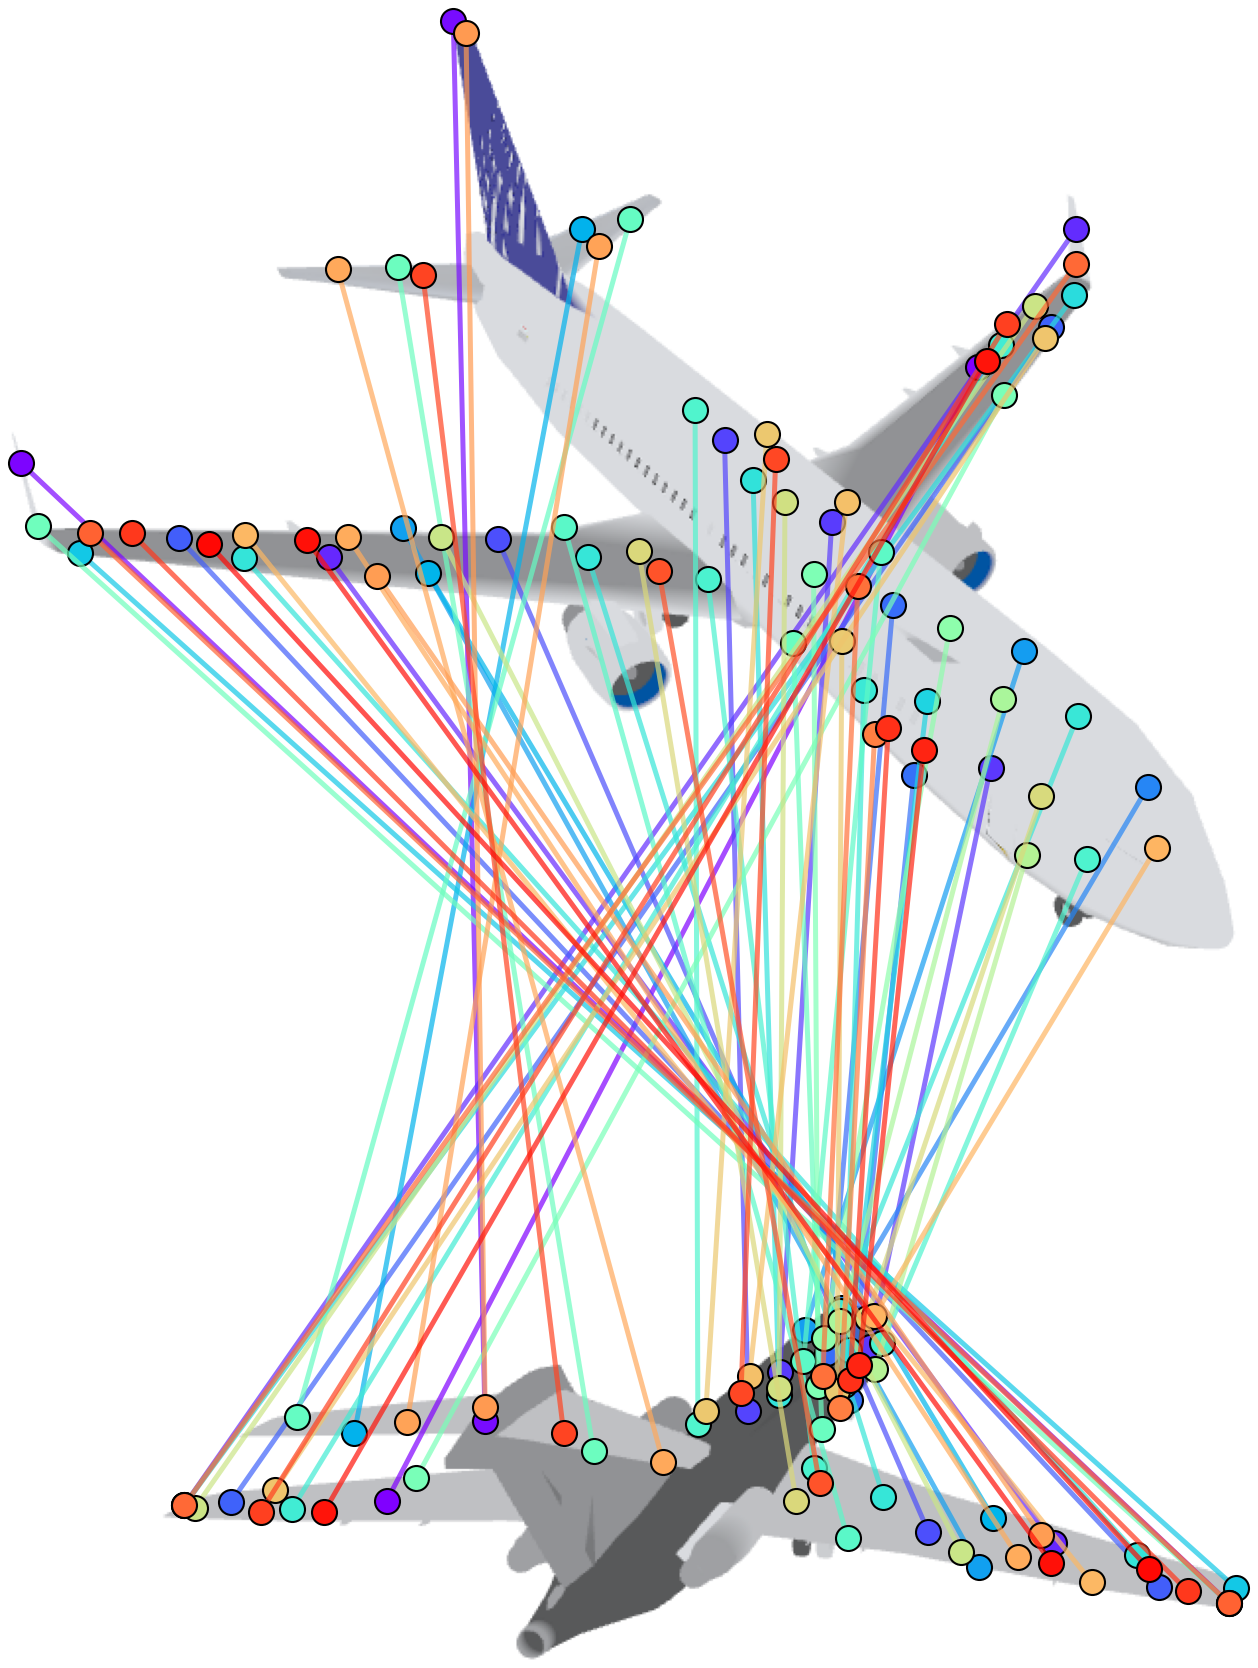
\includegraphics[width=\linewidth,height=11.5cm,keepaspectratio]{images/semgeogen/2d_2d.png}\\[0.2em]
{\Large\textbf{2D--2D}}
\end{minipage}\hfill
\begin{minipage}[t]{0.32\linewidth}
\centering
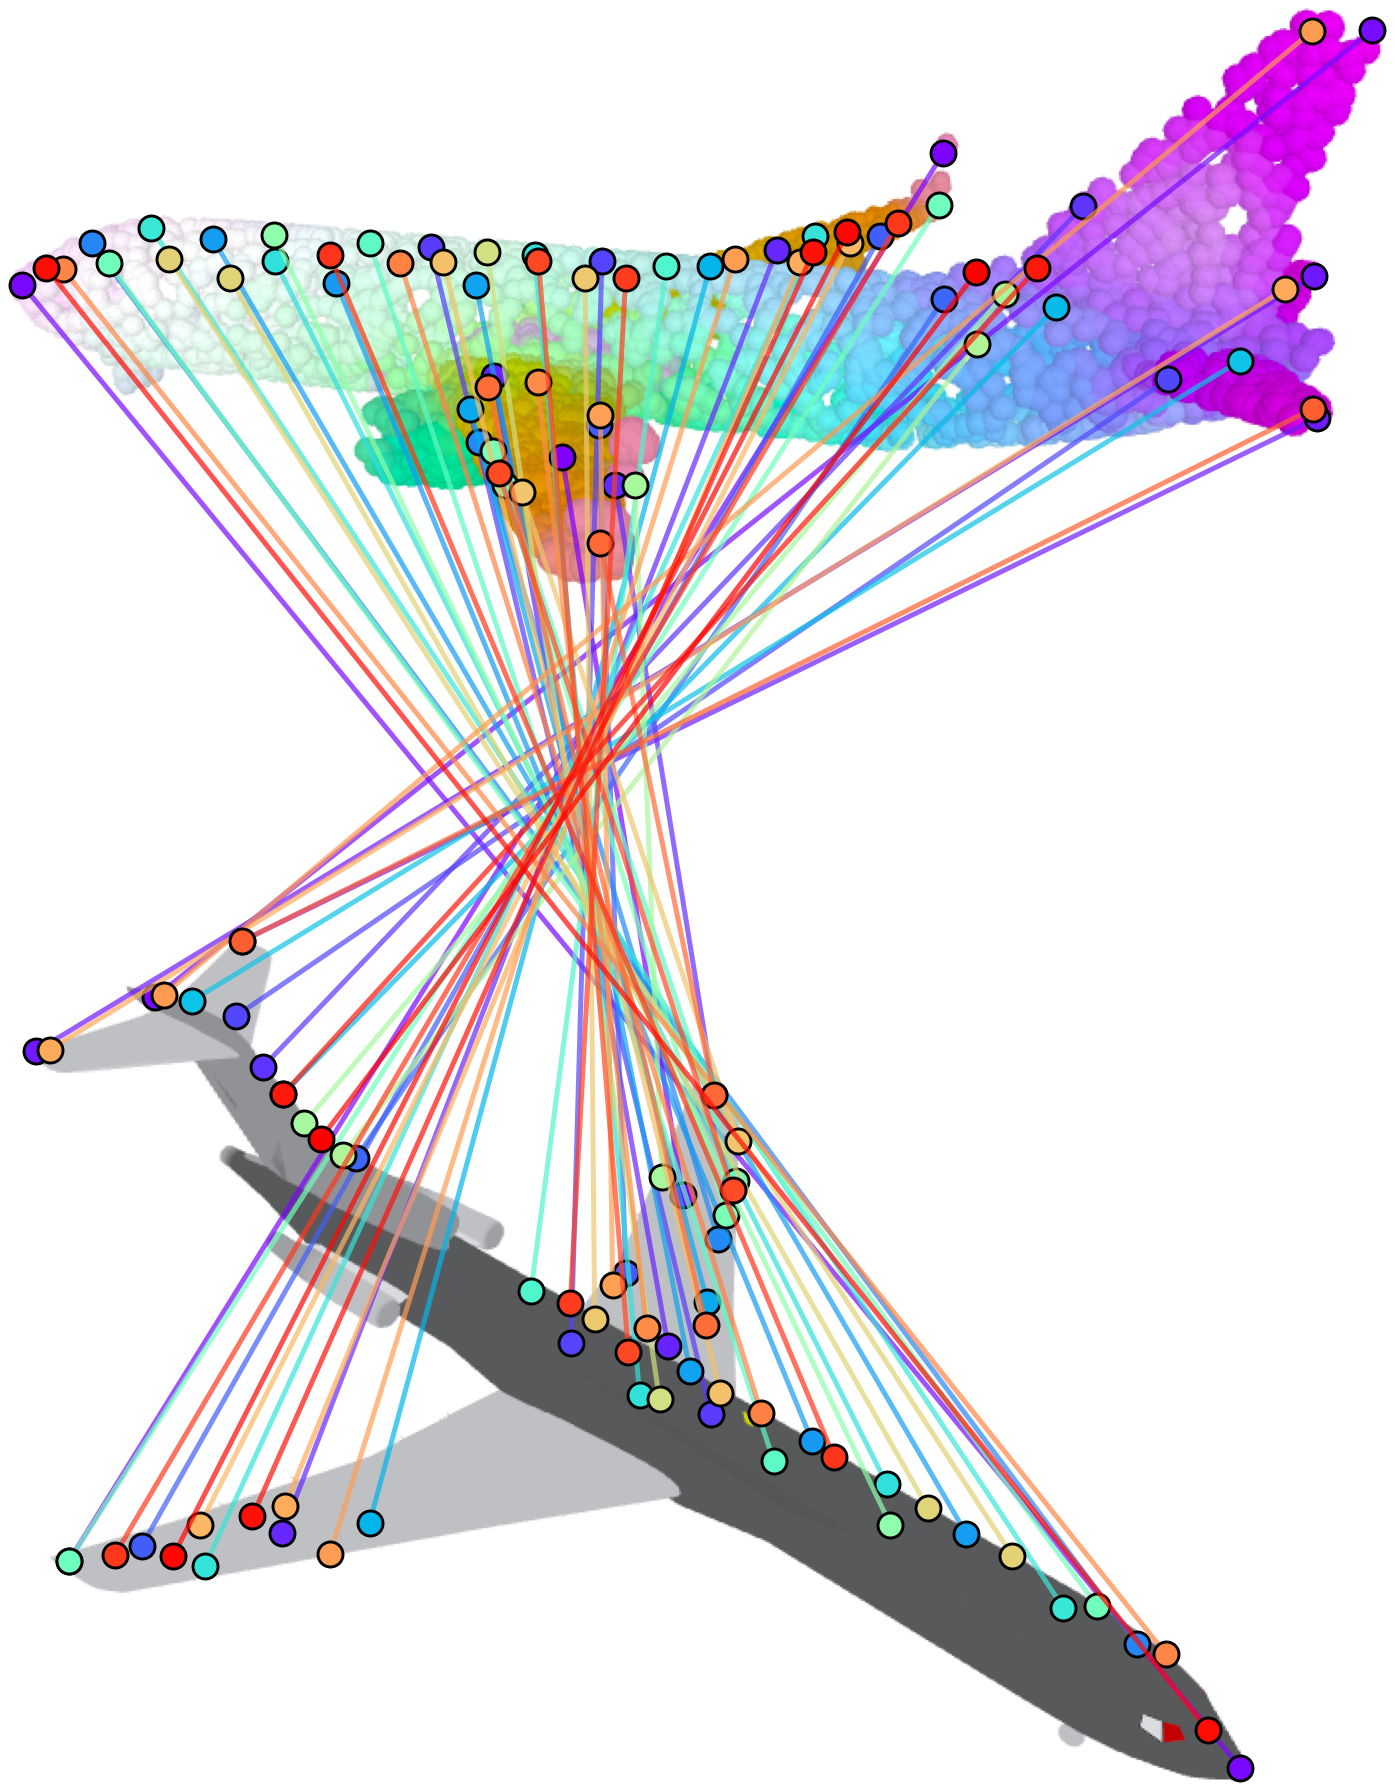
\includegraphics[width=\linewidth,height=11.5cm,keepaspectratio]{images/semgeogen/3d_2d.png}\\[0.2em]
{\Large\textbf{3D--2D}}
\end{minipage}\hfill
\begin{minipage}[t]{0.32\linewidth}
\centering
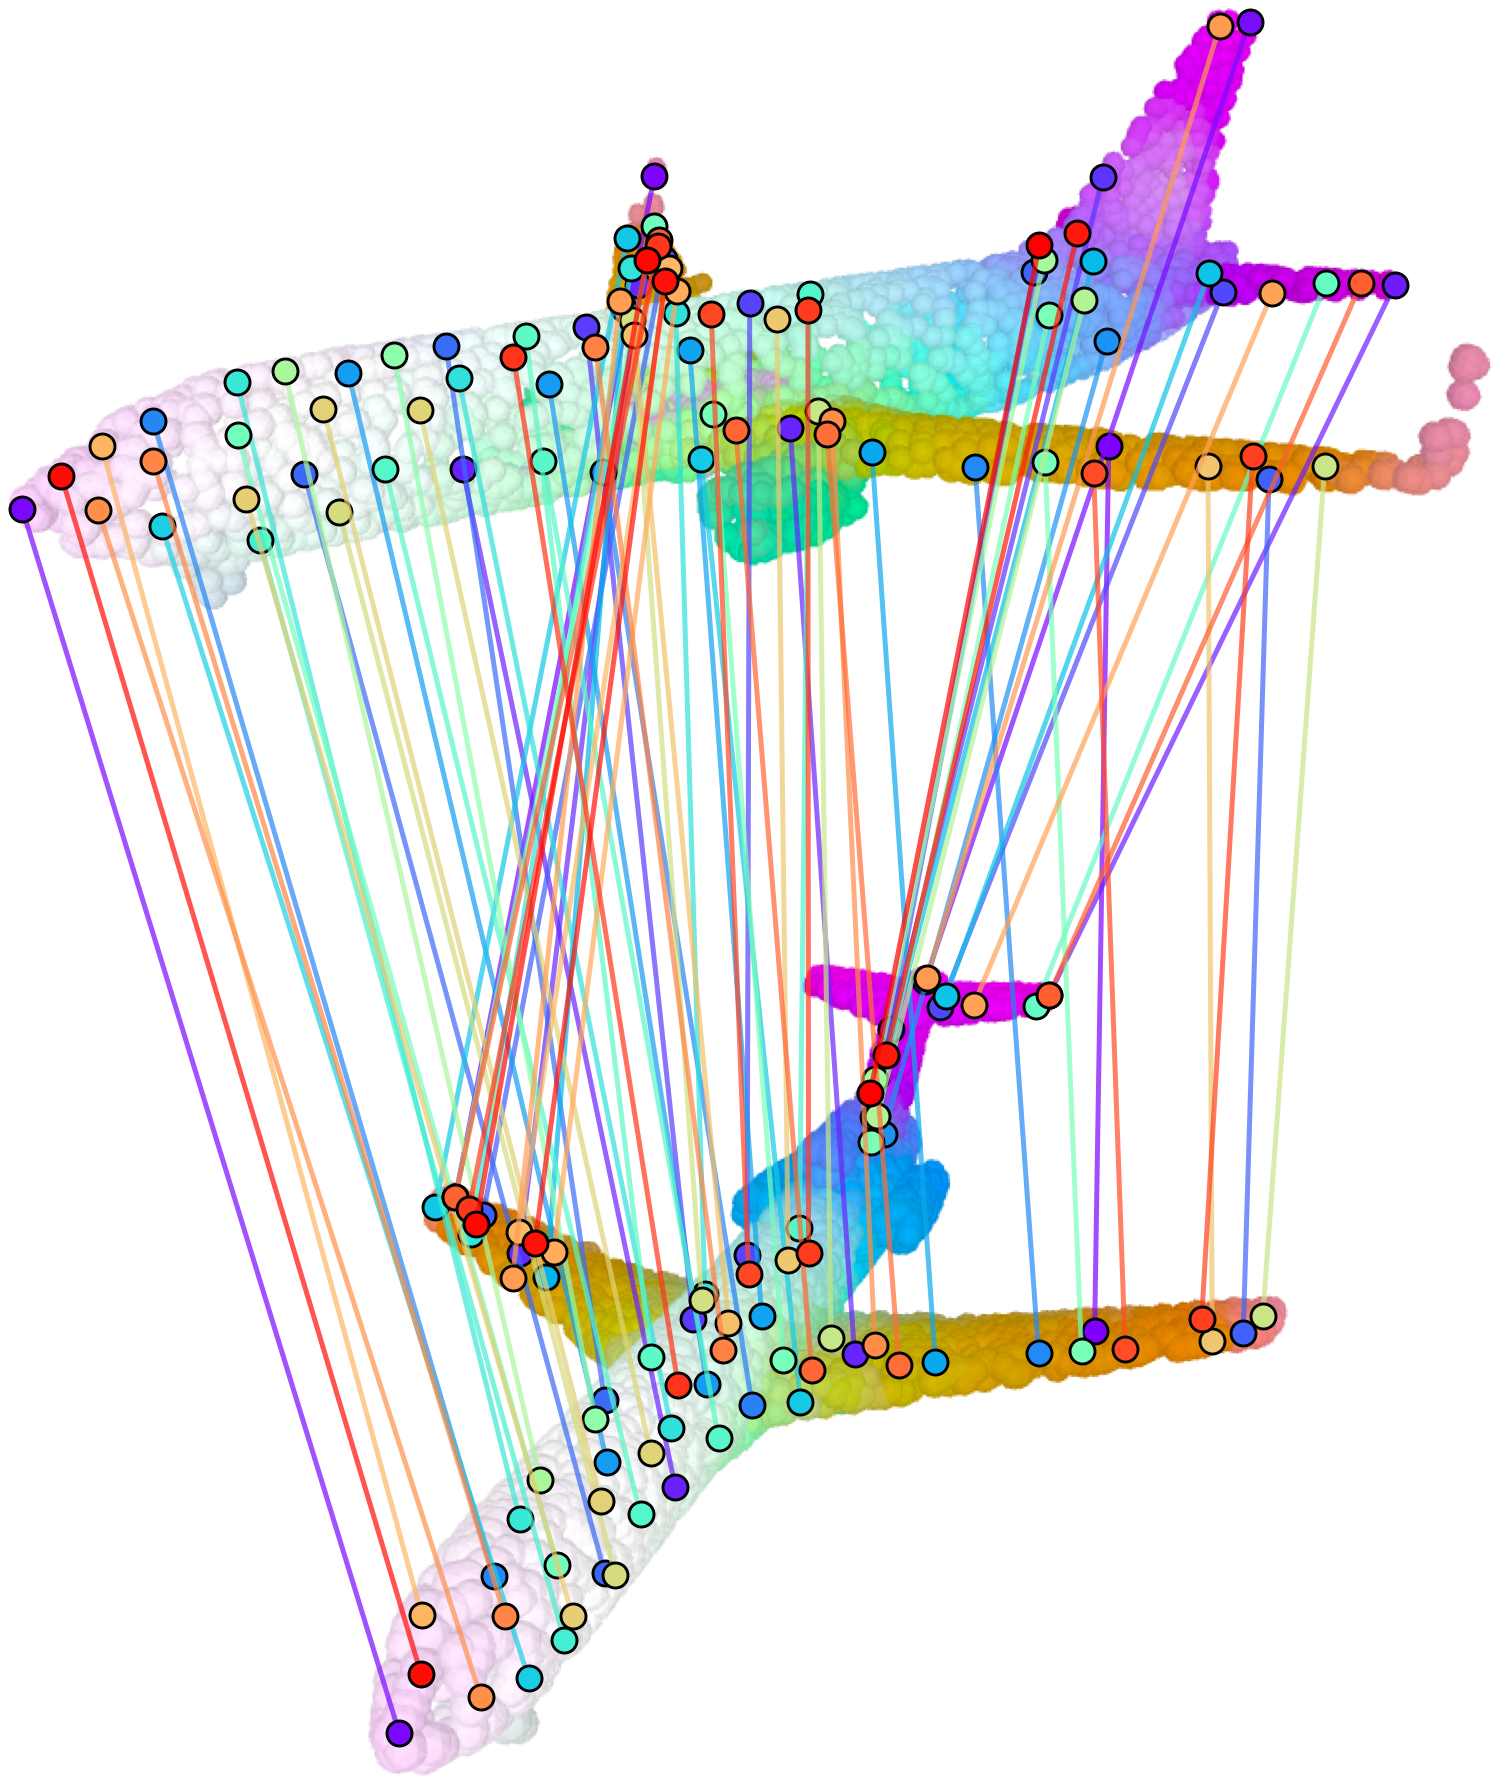
\includegraphics[width=\linewidth,height=11.5cm,keepaspectratio]{images/semgeogen/3d_3d.png}\\[0.2em]
{\Large\textbf{3D--3D}}
\end{minipage}

\vspace{0.3em}
{\large Generated correspondences between two airplane instances across modalities.
3D colors show lifted DINOv2 features (PCA to RGB).}

\vspace{0.6em}
\StatBox{0}{manual labels\\(no point / part / corr.)}\hfill
\StatBox{93\%}{PCK@0.10 vs.\\human KeypointNet}\hfill
\StatBox{+4.4 / +2.9}{SPair-71k mean PCK\\GeoAware-SC / MARCO}
}

\block{\huge\vphantom{Akg}SemGeo-Gen Pipeline}{
\centering
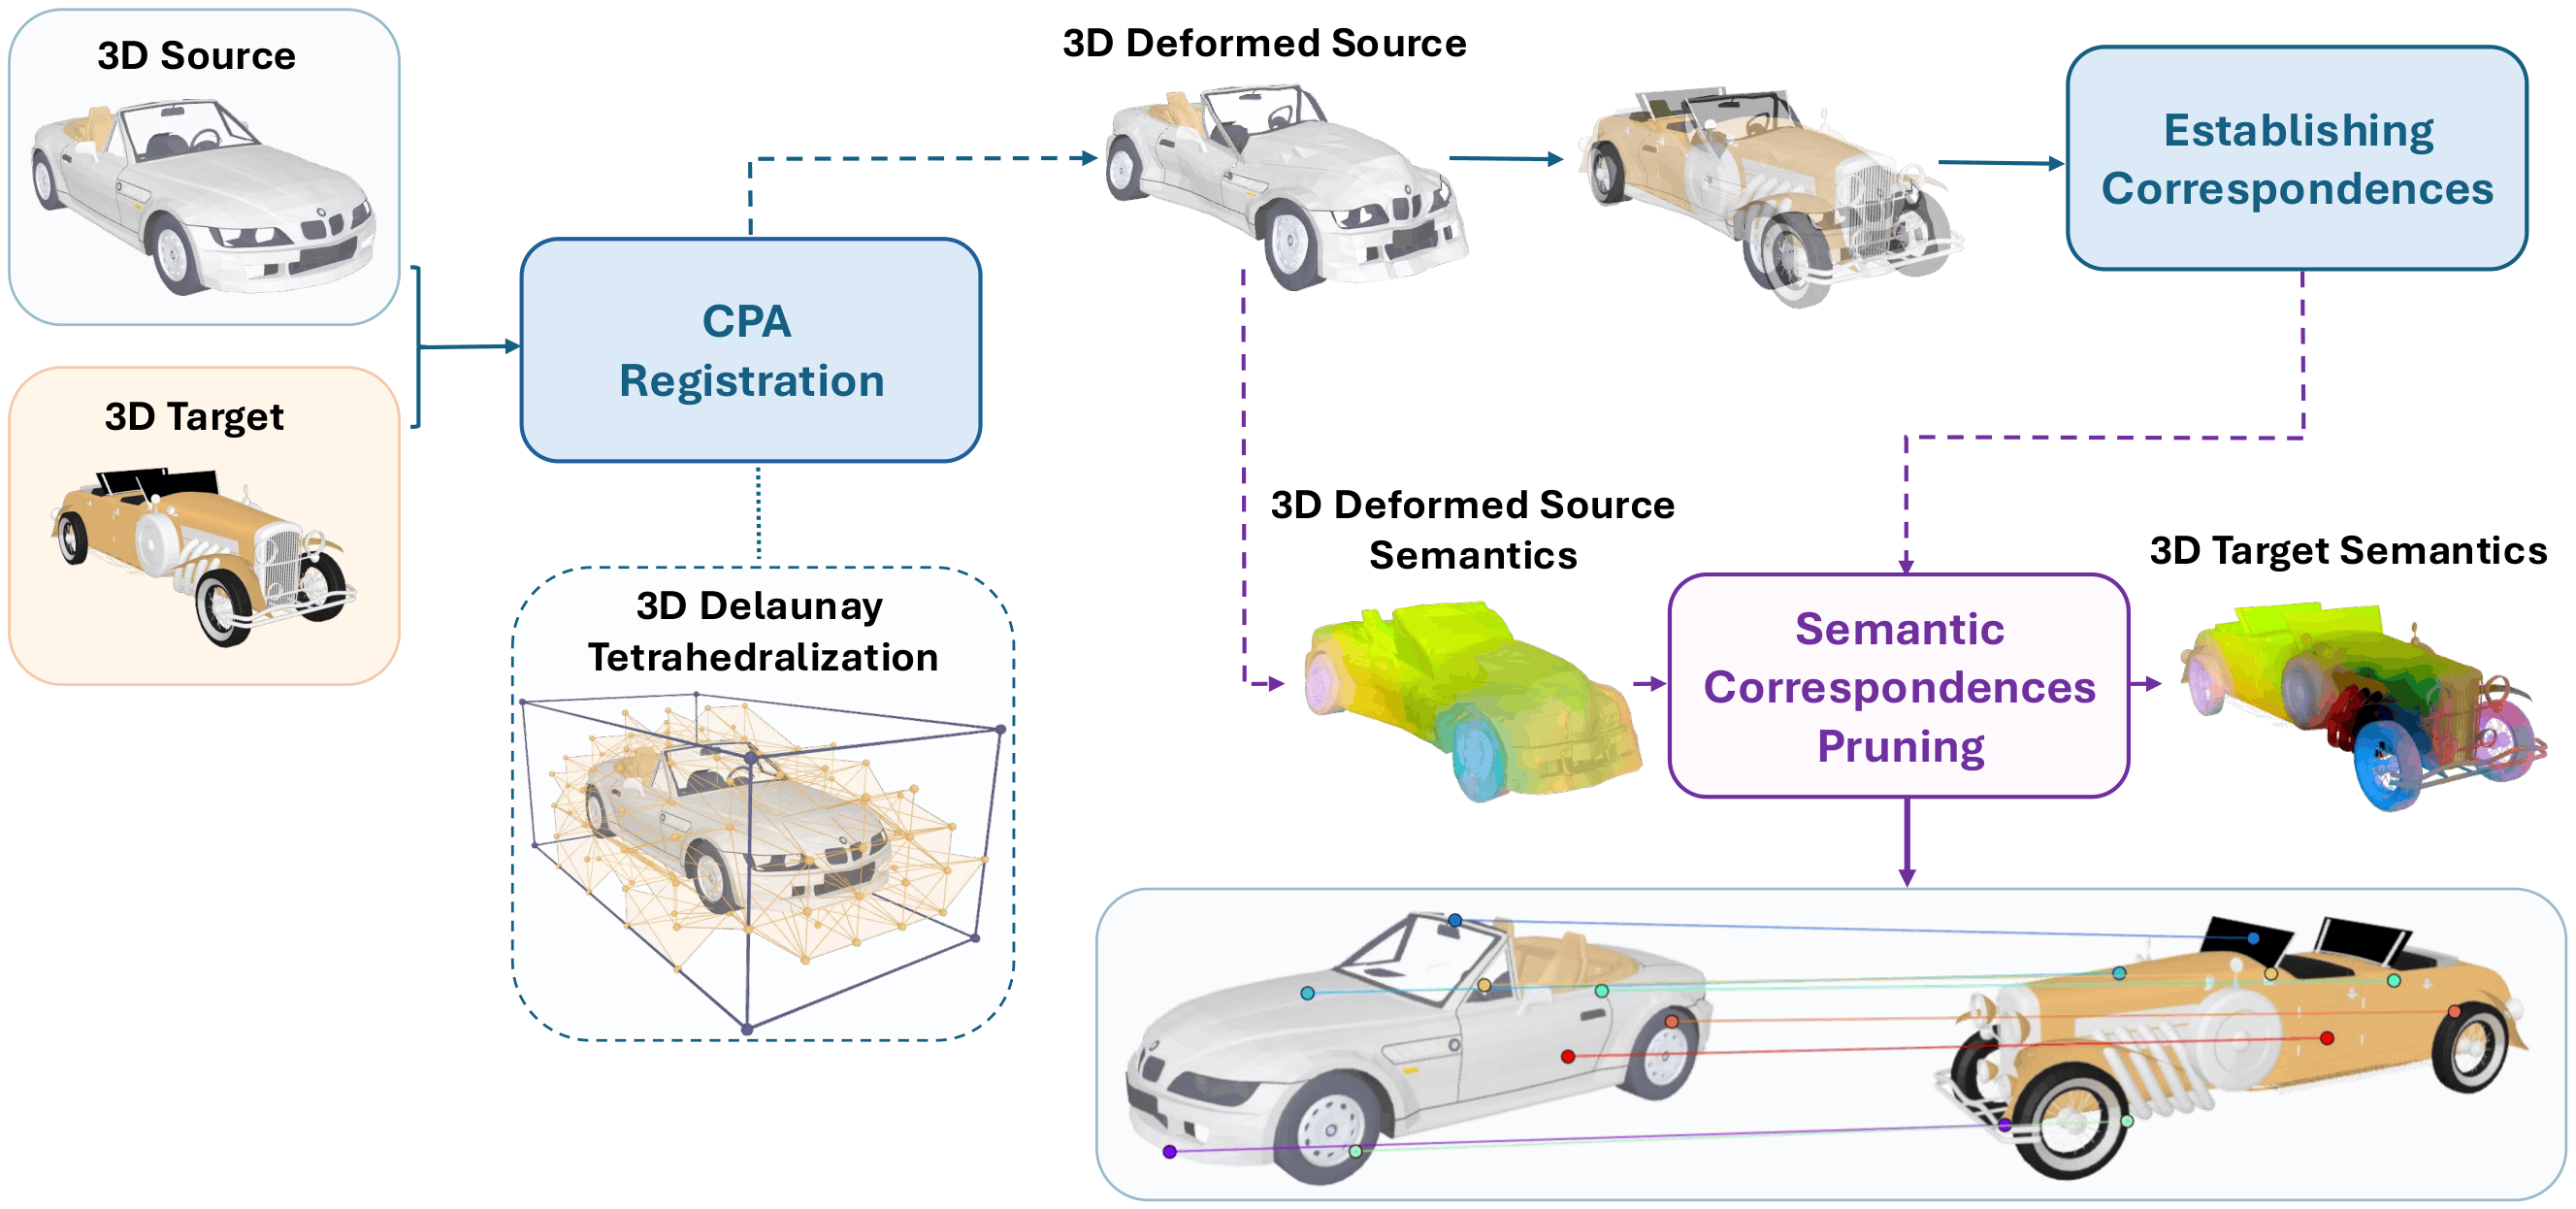
\includegraphics[width=\linewidth,height=17cm,keepaspectratio]{images/semgeogen/powerpoint_full_method.png}

\vspace{0.4em}
\raggedright
\Large
\textbf{Input:} pairs $(\cS,\cT)$ that are only \textbf{rotation-aligned and scale-normalized},
a weak category-level prior with \emph{no} point, part, or correspondence supervision.

\begin{enumerate}[nosep,leftmargin=1.3em,itemsep=0.25em]
    \item \textbf{Lift features:} render multiple views, extract dense DINOv2 features, lift them to 3D points.
    \item \textbf{CPA registration:} non-rigidly deform the source onto the target.
    \item \textbf{Match \& prune:} nearest-neighbor matches, then remove semantically inconsistent ones.
\end{enumerate}
}

\block{\huge\vphantom{Akg}Method}{
\Large
\textbf{Semantic similarity} (joint 64-D PCA of DINOv2 descriptors $z$)
\[
\ssem(x_i,x_j)=\frac{z_i^\top z_j}{\|z_i\|_2\,\|z_j\|_2}>\tsem,
\qquad \tsem=0.85.
\]

\textbf{Continuous piecewise-affine (CPA) registration.}
A Delaunay-tetrahedralized control grid with per-vertex displacements $u_v$ gives a deformation
that is affine inside each tetrahedron and continuous across cells:
\[
\cL_{\mathrm{CPA}}
=\cL_{\mathrm{Chamfer}}\!\big(\TCPA(\cX_S),\cX_T\big)
+\lambda\,\frac{1}{|\mathcal{E}|}\!\sum_{(a,b)\in\mathcal{E}}\!\|u_a-u_b\|_2^2 .
\]

\textbf{Match, then prune.} With $\hat{x}_i^S=\TCPA(x_i^S)$:
\[
a(i)=\arg\min_{j}\|\hat{x}_i^S-x_j^T\|_2,
\qquad
\cC_{\cS,\cT}=\big\{(x_i^S,x_{a(i)}^T)\;:\;\ssem(x_i^S,x_{a(i)}^T)>\tsem\big\}.
\]

\textbf{Project to 2D.} Rendering with cameras $\pi_{c_S},\pi_{c_T}$ turns each 3D match into
3D--2D and 2D--2D supervision: $(u_i^S,u_j^T)=\big(\pi_{c_S}(x_i^S),\pi_{c_T}(x_j^T)\big)$.
$N$ objects give up to $\binom{N}{2}$ pairs, each renderable from many views.
}

\block{\huge\vphantom{Akg}Takeaway}{
\noindent
\begin{minipage}[t]{0.25\linewidth}
\vspace{0pt}
\centering
% TODO: placeholder QR (from the GSA poster) - replace with the SemGeo-Gen QR code

\includegraphics[width=0.85\linewidth]{images/gsa_web_qr_canva.jpeg}
\end{minipage}
\hfill
\begin{minipage}[t]{0.72\linewidth}
\vspace{0pt}
\Large
Approximate semantic-geometric correspondences generated from 3D assets, \textbf{without manual correspondence annotation},
are a scalable training signal that improves real-image semantic correspondence.

\vspace{0.4em}
\large
Scan for paper, code, and generated data.
\end{minipage}
}


% ============================================================
% RIGHT COLUMN
% ============================================================
\column{0.49}

\block{\huge\vphantom{Akg}Pretraining Boosts SPair-71k}{
\Large
Pretrain on our generated 2D pairs (12K per category, Objaverse-OA), then fine-tune on real SPair-71k.
\textbf{No architectural changes.}

\vspace{0.3em}
\centering
{\large Recent supervised SOTA methods under different training regimes. PCK@0.10 $\uparrow$. P.T.\ = pretraining.}\par
\vspace{0.2em}
\renewcommand{\arraystretch}{1.3}
\setlength{\tabcolsep}{5pt}
\resizebox{\linewidth}{!}{%
\begin{tabular}{llccccccccc|c}
\toprule
\textbf{Method} & \textbf{Training} & \textbf{aero} & \textbf{bike} & \textbf{boat} & \textbf{bus} & \textbf{car} & \textbf{chair} & \textbf{mbike} & \textbf{train} & \textbf{tv} & \textbf{Mean} \\
\midrule
\multirow{3}{*}{GeoAware-SC}
& SPair-71k & 83.42 & 71.07 & 66.68 & 90.93 & 86.10 & 62.18 & 79.54 & 95.33 & 79.00 & 79.36 \\
& SPair-71k + Ours & 86.28 & 74.60 & 68.33 & 93.12 & 84.73 & 68.94 & 79.73 & 95.31 & 80.73 & 81.31 \\
\rowcolor{oursrow}
& Ours P.T.\,$\rightarrow$\,SPair & \textbf{89.38} & \textbf{76.11} & \textbf{71.15} & \textbf{93.80} & \textbf{86.74} & \textbf{73.80} & \textbf{82.33} & \textbf{95.67} & \textbf{84.59} & \textbf{83.73} \\
\midrule
\multirow{3}{*}{MARCO}
& SPair-71k & 92.16 & 76.76 & 76.53 & 93.17 & 88.57 & 82.49 & 82.03 & 93.62 & 91.72 & 86.39 \\
& SPair-71k + Ours & 92.26 & 77.49 & 73.74 & 92.59 & 84.86 & 82.71 & 79.78 & 93.22 & 89.72 & 85.23 \\
\rowcolor{oursrow}
& Ours P.T.\,$\rightarrow$\,SPair & \textbf{95.59} & \textbf{80.66} & \textbf{79.35} & \textbf{94.59} & \textbf{91.89} & \textbf{91.16} & \textbf{82.30} & \textbf{94.69} & \textbf{93.49} & \textbf{89.28} \\
\bottomrule
\end{tabular}}

\vspace{0.7em}
{\Large\textbf{MARCO: SPair-71k only (top) vs.\ Ours P.T.\,$\rightarrow$\,SPair-71k (bottom)}}\par
\vspace{0.3em}
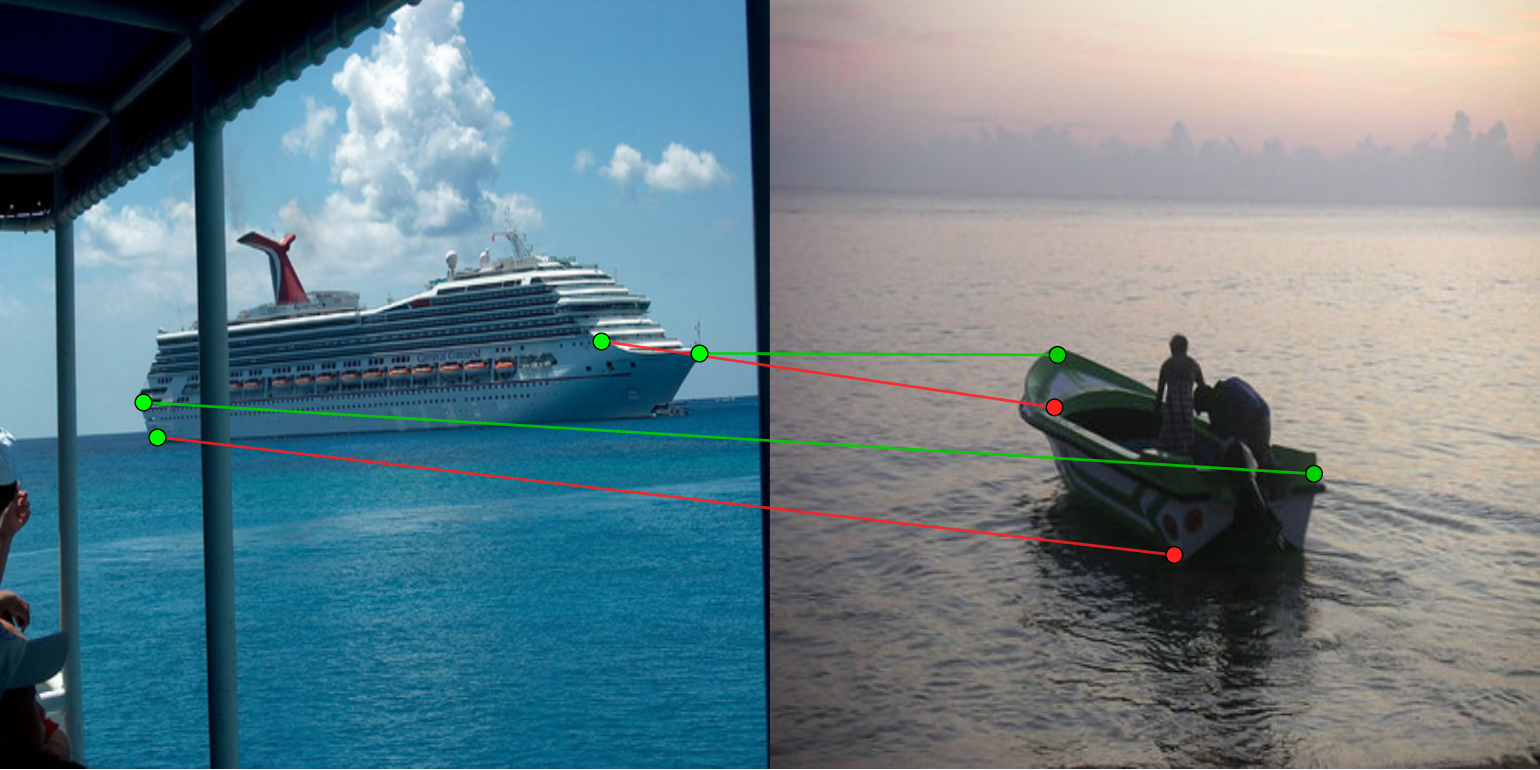
\includegraphics[width=0.325\linewidth]{images/semgeogen/match_real_boat.png}\hfill
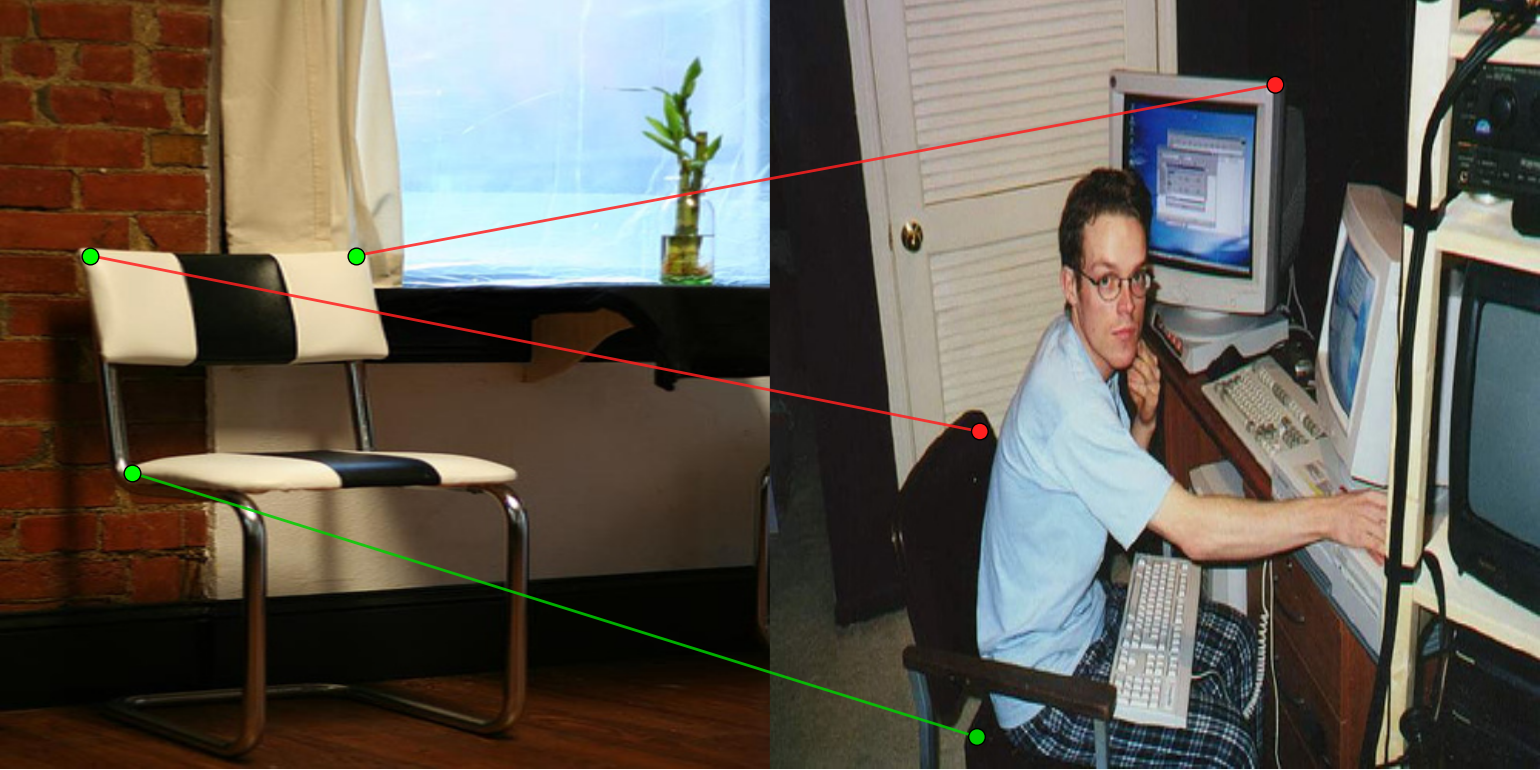
\includegraphics[width=0.325\linewidth]{images/semgeogen/match_real_chair.png}\hfill
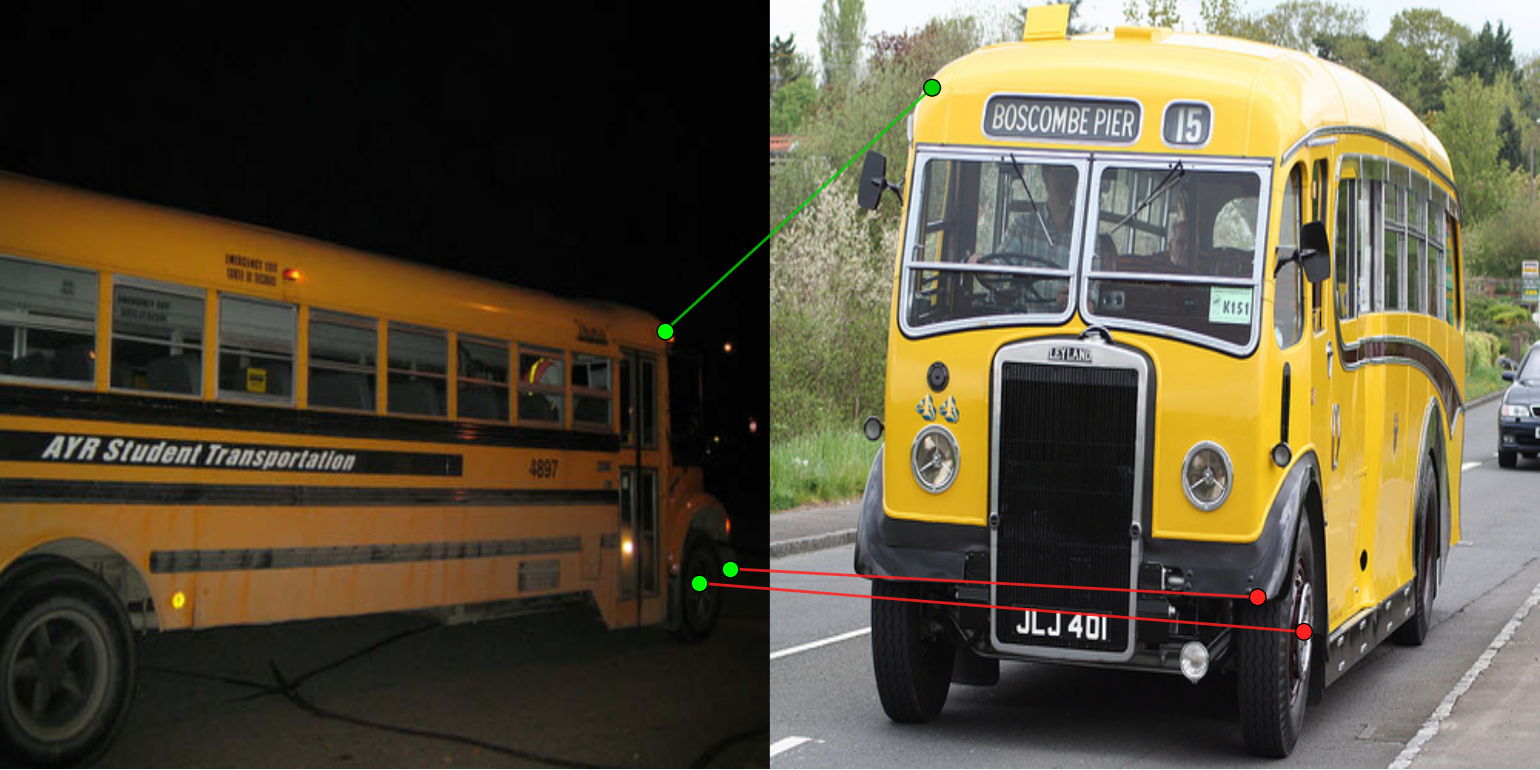
\includegraphics[width=0.325\linewidth]{images/semgeogen/match_real_bus.png}\\[0.25em]
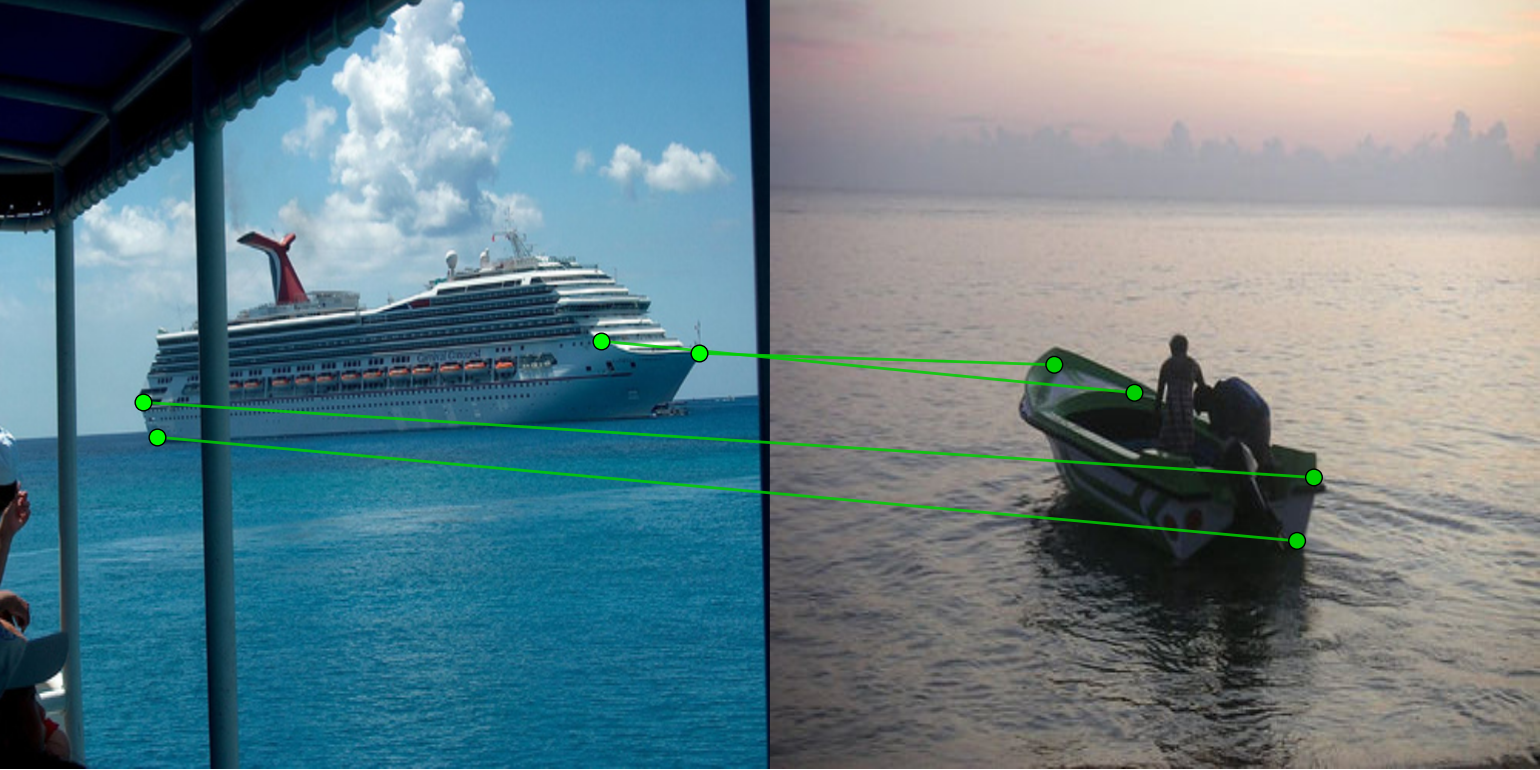
\includegraphics[width=0.325\linewidth]{images/semgeogen/match_ours_boat.png}\hfill
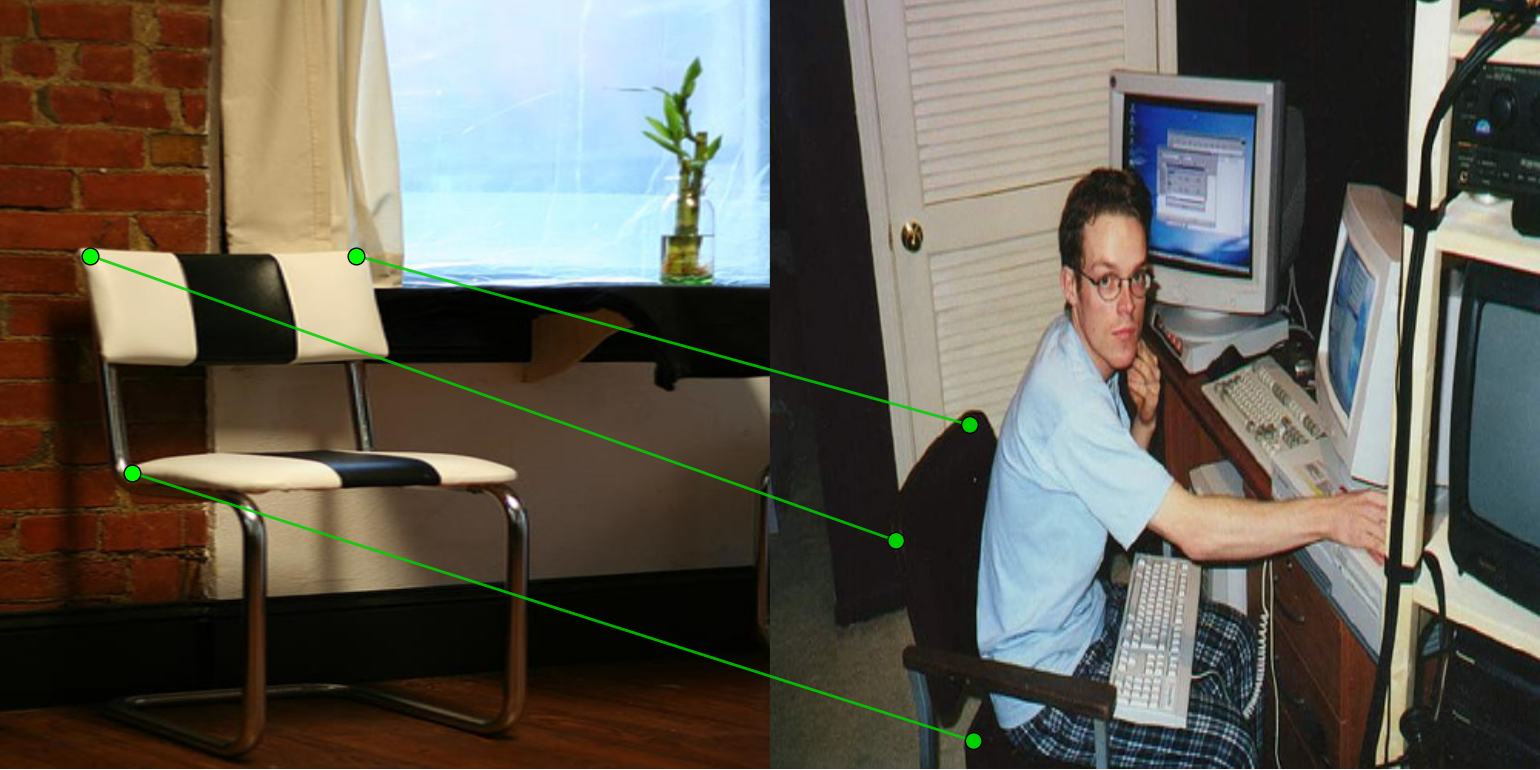
\includegraphics[width=0.325\linewidth]{images/semgeogen/match_ours_chair.png}\hfill
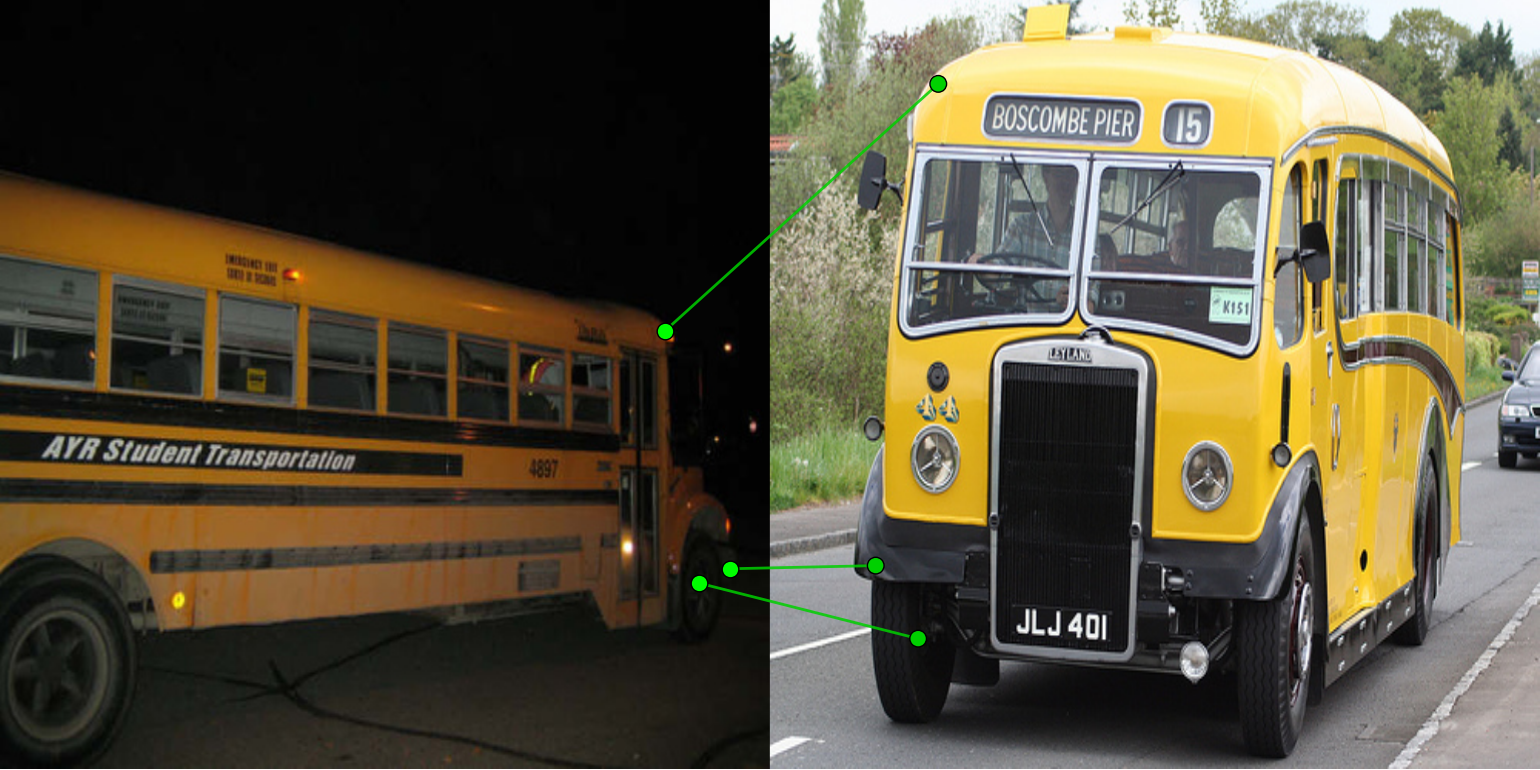
\includegraphics[width=0.325\linewidth]{images/semgeogen/match_ours_bus.png}

\vspace{0.2em}
{\large \textcolor{KellyGreen}{\textbf{Green}}: correct match; \textcolor{Red}{\textbf{red}}: wrong match.}
}

\block{\huge\vphantom{Akg}Semantic Coverage \& Pruning}{
\centering
\makebox[0.98\linewidth]{%
    \makebox[0.333\linewidth][c]{\large\textbf{Rendering}}%
    \makebox[0.333\linewidth][c]{\large\textbf{Joint DINOv2 PCA}}%
    \makebox[0.333\linewidth][c]{\large\textbf{Semantic coverage}}%
}\\[0.2em]
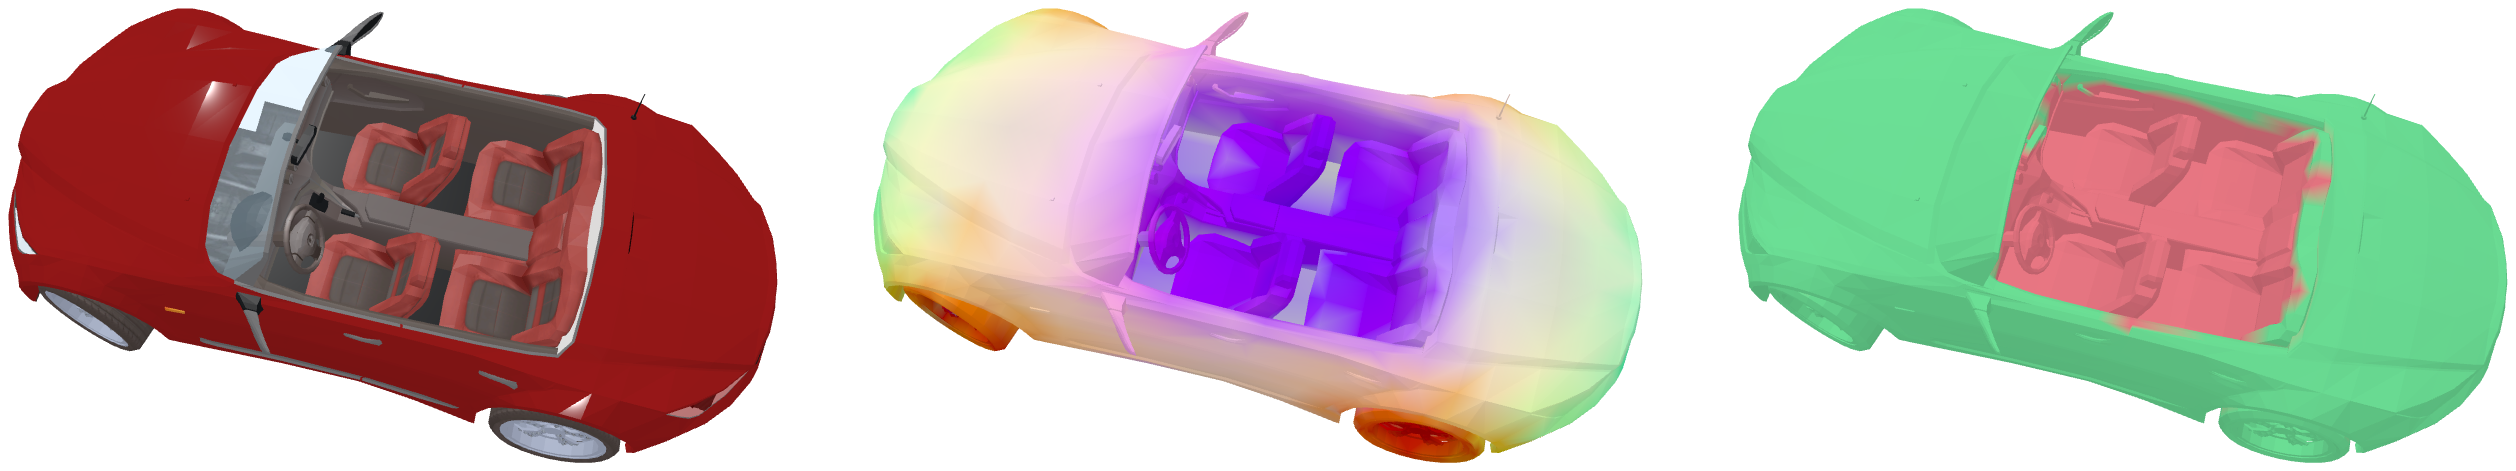
\includegraphics[width=0.98\linewidth]{images/semgeogen/src_triplet_view2.png}\\[0.3em]
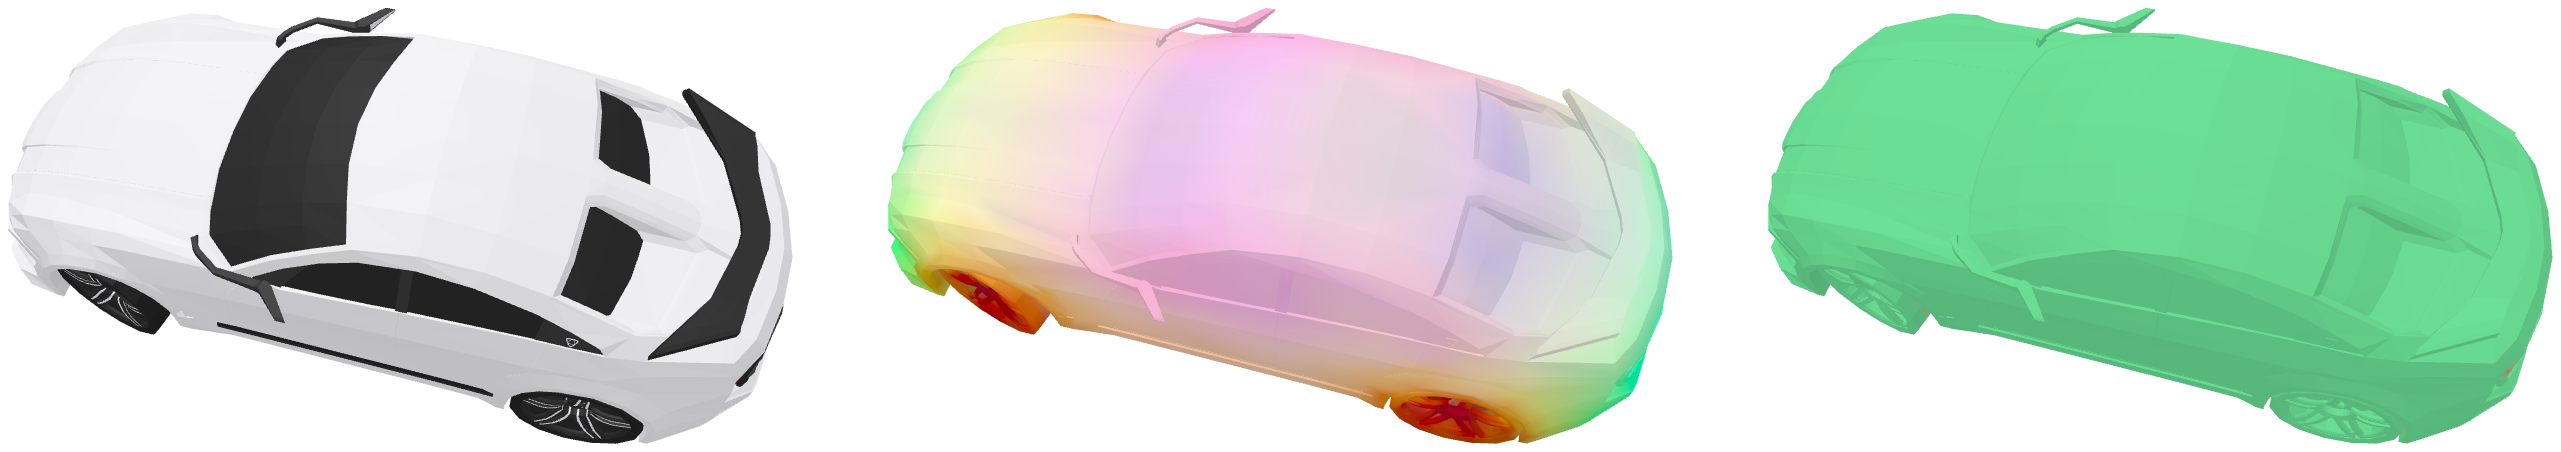
\includegraphics[width=0.98\linewidth]{images/semgeogen/tgt_triplet_view2.png}

\vspace{0.3em}
\raggedright
\Large
\textcolor{KellyGreen}{\textbf{Green}}: has a semantic match in the paired object; \textcolor{Red}{\textbf{red}}: none (exposed seats)
and never gets correspondences. Pairs with low coverage ($\rho_{\mathrm{sem}}<0.6$) are optionally filtered.

\vspace{0.5em}
\centering
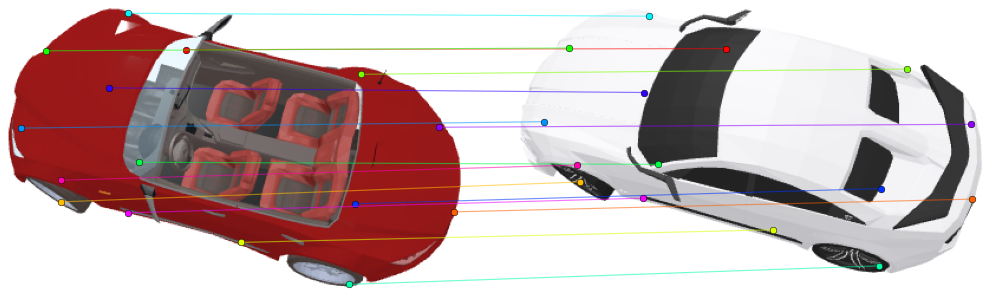
\includegraphics[width=0.52\linewidth]{images/semgeogen/sparse15_view10.png}\par
\vspace{0.2em}
{\large Final correspondences: seats, steering wheel, and the white roof get no matches.}
}

\block{\huge\vphantom{Akg}Agreement with Human Annotations}{
\Large
Generated 3D matches vs.\ human keypoints on \textbf{KeypointNet} (evaluation only).

\vspace{0.3em}
\centering
\renewcommand{\arraystretch}{1.2}
\setlength{\tabcolsep}{4pt}
\resizebox{\linewidth}{!}{%
\begin{tabular}{l*{16}{c}|>{\columncolor{oursrow}}cc}
\toprule
\textbf{PCK} & Aero & Bath & Bed & Bottle & Cap & Car & Chair & Guitar & Helmet & Knife & Laptop & Motor & Mug & Skate & Table & Vessel & \textbf{Mean} & \textbf{Median} \\
\midrule
@0.05 & 0.79 & 0.70 & 0.68 & 0.83 & 0.80 & 0.78 & 0.77 & 0.81 & 0.55 & 0.83 & 0.89 & 0.75 & 0.73 & 0.86 & 0.76 & 0.45 & \textbf{0.75} & 0.78 \\
@0.10 & 0.94 & 0.88 & 0.91 & 0.96 & 0.97 & 0.95 & 0.96 & 0.96 & 0.84 & 0.93 & 0.99 & 0.93 & 0.96 & 0.97 & 0.96 & 0.71 & \textbf{0.93} & 0.96 \\
@0.15 & 0.98 & 0.96 & 0.96 & 0.98 & 1.00 & 0.99 & 0.99 & 0.98 & 0.94 & 0.96 & 1.00 & 0.98 & 0.99 & 0.99 & 0.99 & 0.87 & \textbf{0.97} & 0.98 \\
@0.20 & 0.99 & 0.99 & 0.99 & 0.99 & 1.00 & 1.00 & 0.99 & 0.99 & 0.98 & 0.98 & 1.00 & 0.99 & 1.00 & 1.00 & 1.00 & 0.94 & \textbf{0.99} & 0.99 \\
\bottomrule
\end{tabular}}

\vspace{0.8em}
\begin{minipage}[t]{0.40\linewidth}
\centering
{\Large\textbf{Semantic filtering}}\par
\vspace{0.2em}
\large
\begin{tabular}{lc}
\toprule
\textbf{Setting} & \textbf{PCK@.10} \\
\midrule
Geometry only & 0.84 \\
+ corr.\ pruning & 0.91 \\
\rowcolor{oursrow}
+ pair filtering & \textbf{0.93} \\
\bottomrule
\end{tabular}
\end{minipage}\hfill
\begin{minipage}[t]{0.57\linewidth}
\centering
{\Large\textbf{Registration model}}\par
\vspace{0.2em}
\large
\setlength{\tabcolsep}{6pt}
\begin{tabular}{lccc}
\toprule
\textbf{Model} & \textbf{s/pair} & \textbf{PCK@.05} & \textbf{PCK@.10} \\
\midrule
Affine & 1.15 & 0.686 & 0.898 \\
TPS & 3.71 & \textbf{0.739} & 0.919 \\
\rowcolor{oursrow}
\textbf{CPA (ours)} & \textbf{1.13} & 0.729 & \textbf{0.922} \\
\bottomrule
\end{tabular}
\end{minipage}
}

\block{\huge\vphantom{Akg}Beyond Existing Datasets}{
\Large
Correspondences generated on Objaverse-OA categories not covered by existing correspondence datasets.

\vspace{0.3em}
\centering
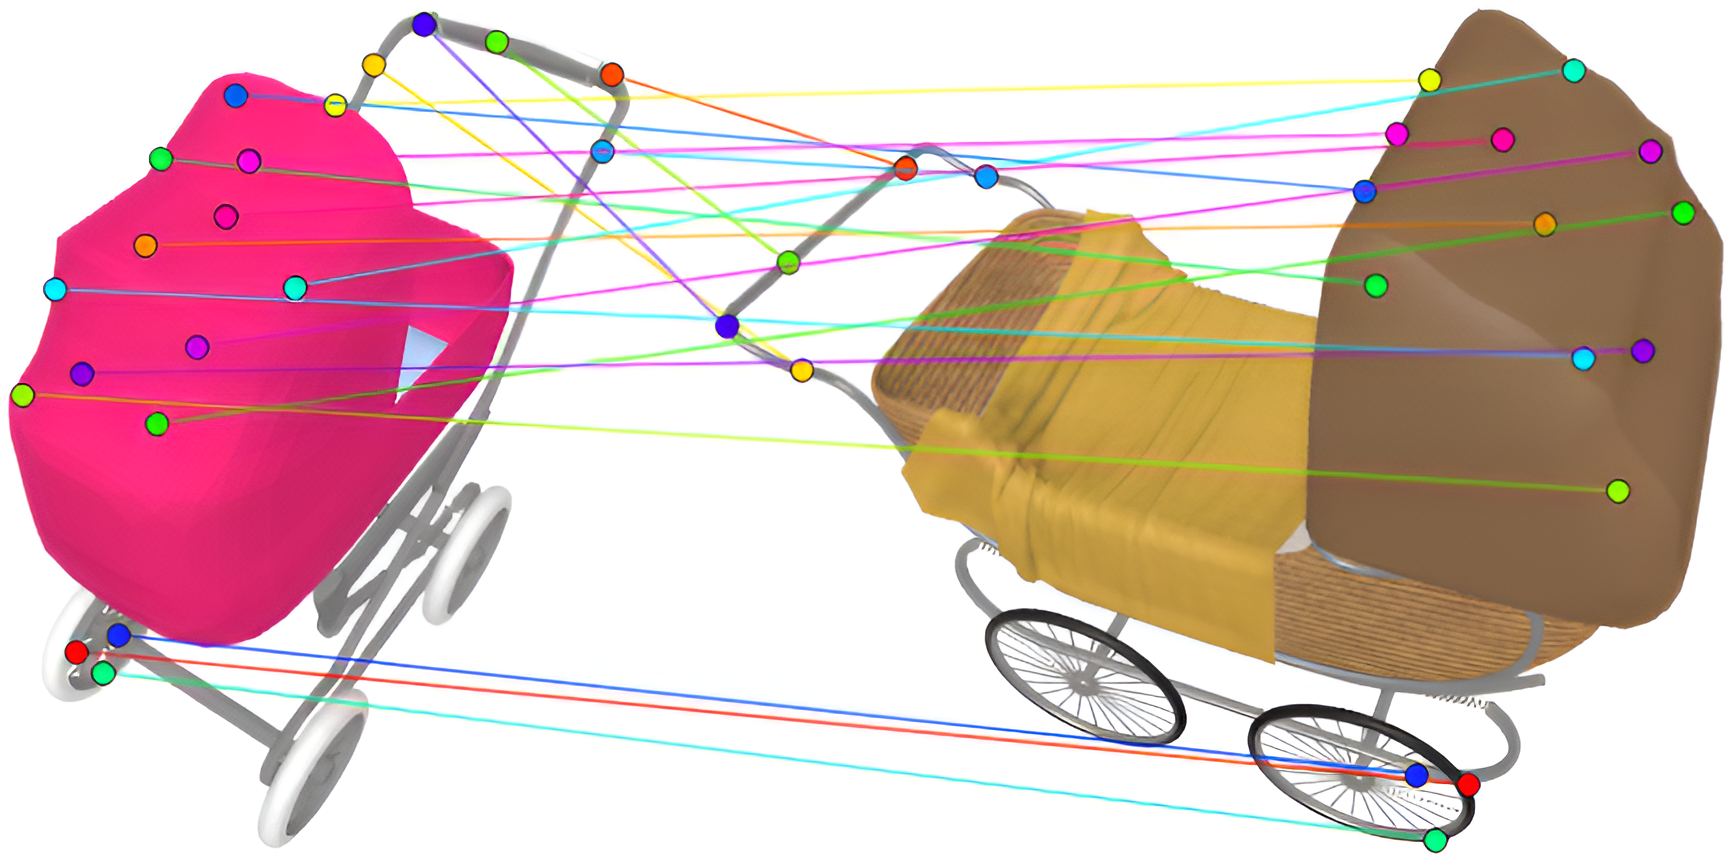
\includegraphics[width=0.36\linewidth,height=8.6cm,keepaspectratio]{images/semgeogen/baby_buggy_highres.png}\hfill
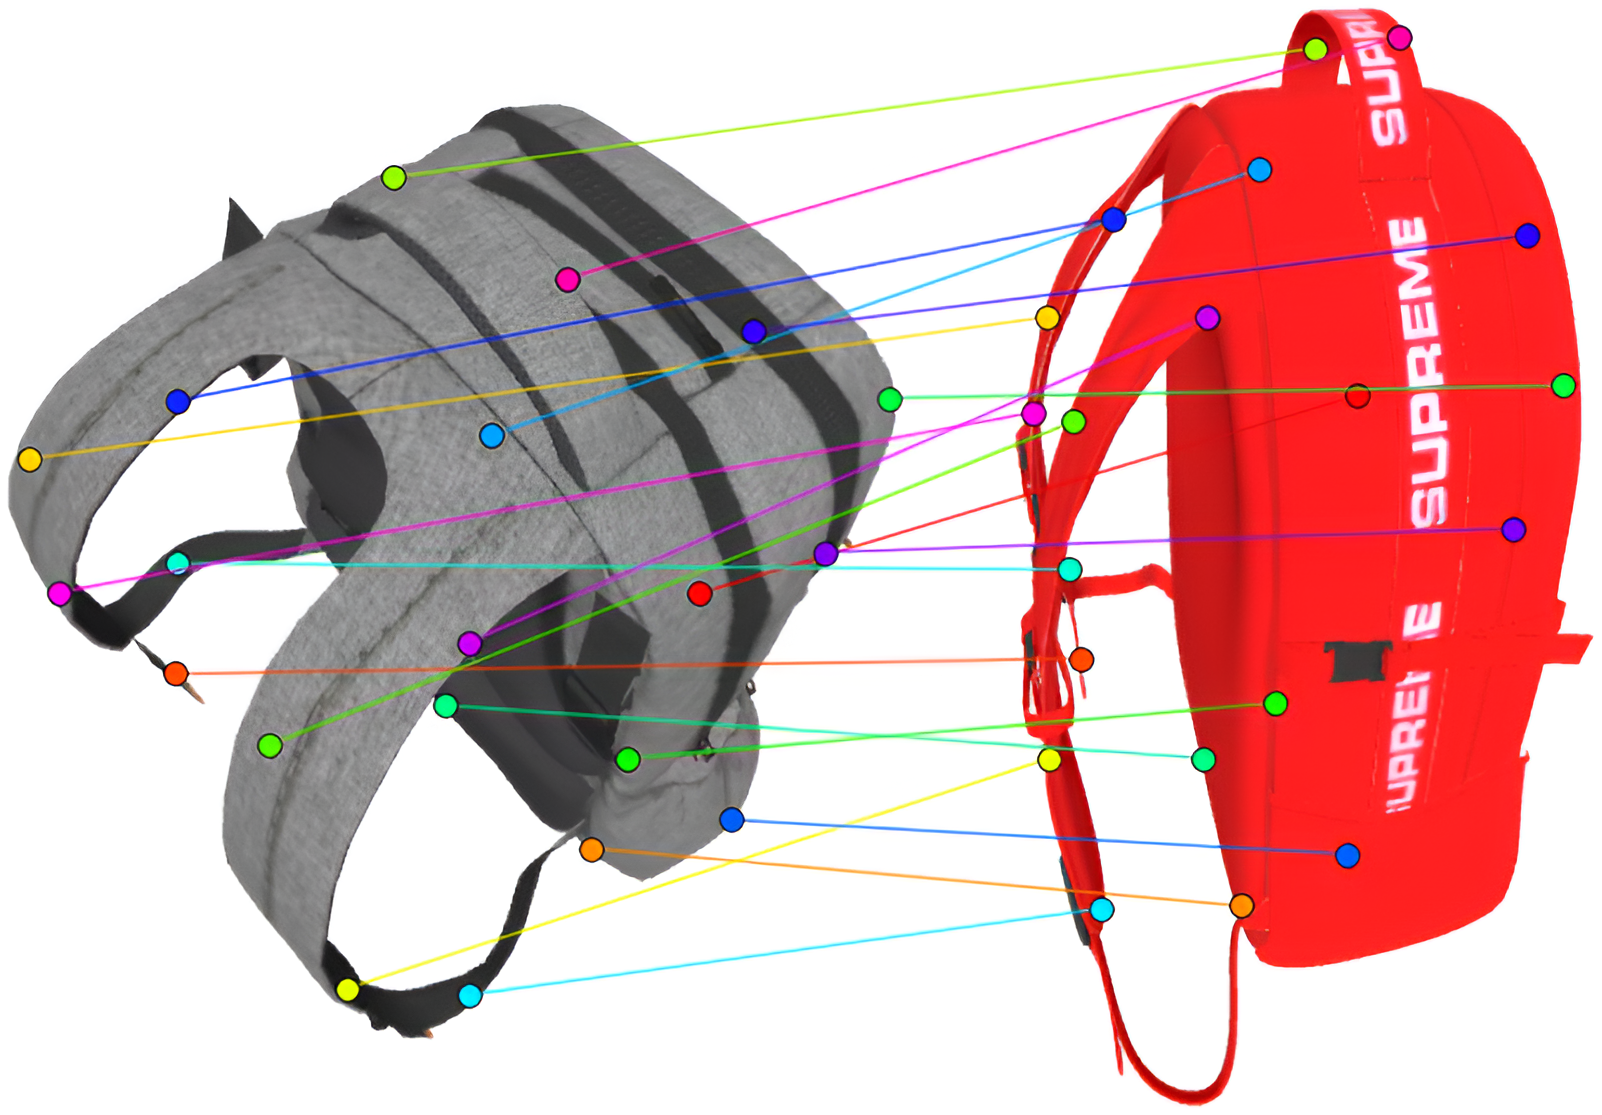
\includegraphics[width=0.29\linewidth,height=8.6cm,keepaspectratio]{images/semgeogen/backpack_highres.png}\hfill
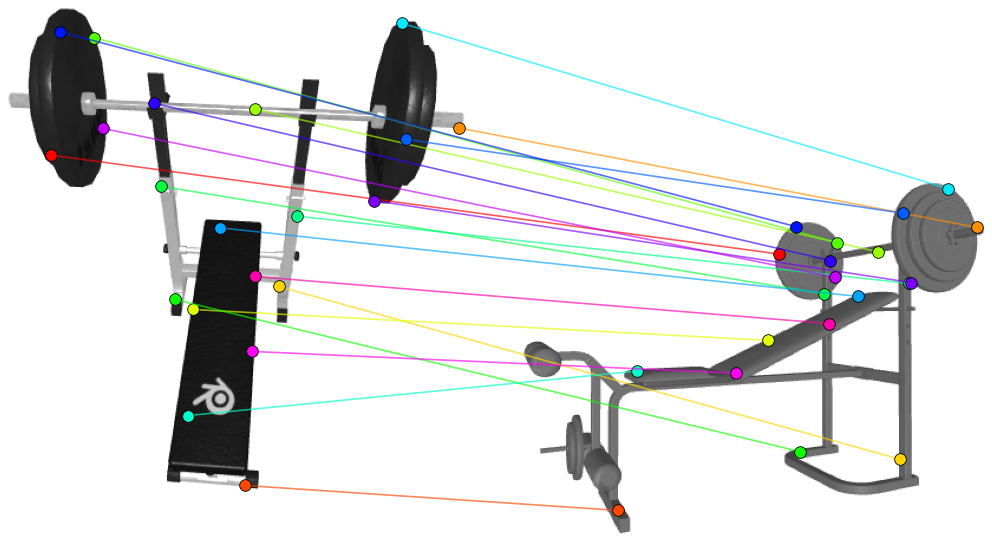
\includegraphics[width=0.33\linewidth,height=8.6cm,keepaspectratio]{images/semgeogen/barbell.png}
}

\end{columns}
\end{document}
